\chapter{Framework Architecture}
The repro-tools \todo{name subject to change } is a framework developed for analysing the reproducibility issues occuring in the neuroimaging pipelines. Though this framework is developed with neuroimaging in focus, it can be used to analyze files belonging to any discipline. In this particular usecase, the HCP data containing the neuroimaging data processed under different conditions is analyzed. The term `condition` here refers to different operating system on which the processing takes place. Under an ideal scenario, different HCP subjects, irrespective of the condition under which the processing takes place, are supposed to have identical checksum. Repro-tools help in identifying the files having differences by comparing the checksum values. It can also quantify these differences with the help of metrics like sum of squared distances (SSD), normalized root mean square error (NRMSE) etc. Repro-tools can also trace the provenance of these differences with the help of data captured by Reprozip.

\begin{center}
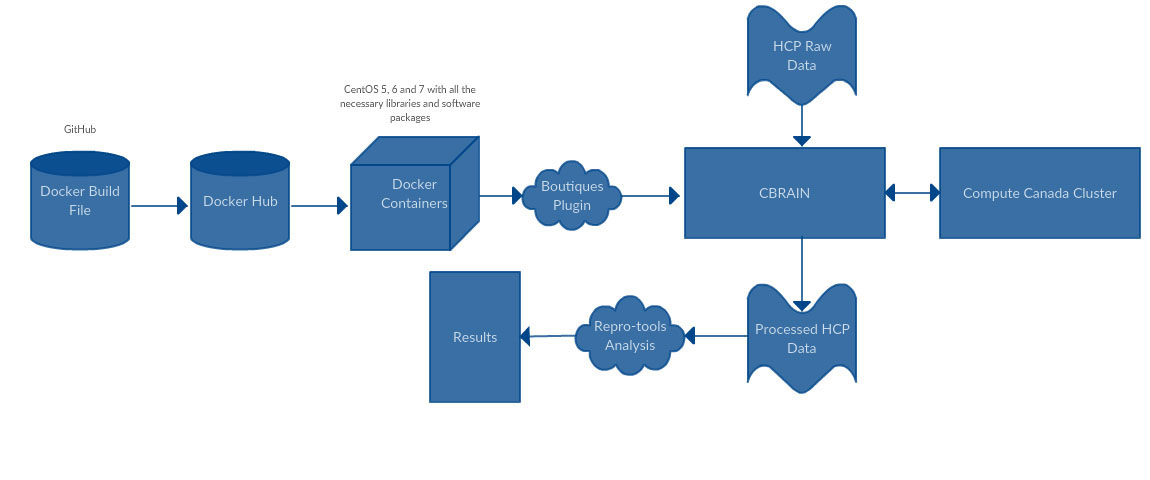
\includegraphics[width=\linewidth]{framework_architecture.jpg}
\captionof{figure}{Framework Architecture}
\label{fig:framework_architecture}
\end{center}

  \begin{itemize}
  \item Collecting data from the Human Connectome Preprocessing Pipelines~\cite{DBHumanConnectome}
  \item Creation of docker images containing the HCP Preprocessing pipelines
  \item Deploying the docker images with the help of Boutiques (A cross-platform application repository for data-analysis platforms) to CBRAIN
  \item Processing of HCP data set using pipelines and measures to check file corruption, recording the software and hardware specifications, provenance capture
  \item Analysis of processed HCP data
  \end{itemize}

\section{Pipeline Containerization}
A container is a self-contained, ready-to-use software component with all the necessary dependencies and softwares~\cite{7158965}. Figure~\ref{fig:container_architecture} illustrates the container image architecture. The architecture is based on LXC which makes use of  cgroups and namespaces. The images are layered on top of each other and the writable container image is kept at the top. The top layer is executable and it can have a state. The container can be considered as a directory containing everything needed for exectuion of an application~\cite{7158965}.\\

\begin{center}
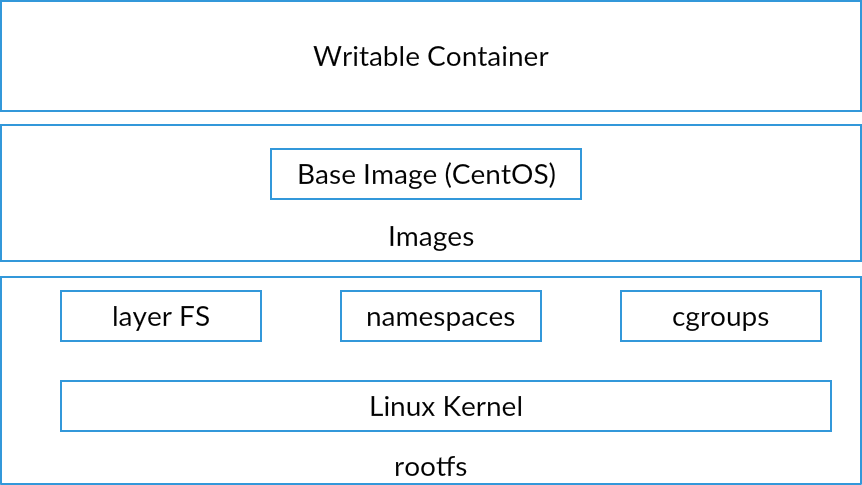
\includegraphics[width=\linewidth]{container_architecture_unedit.png}
\captionof{figure}{Container Architecture}
\label{fig:container_architecture}
\end{center}

Namespace isolation prevents processes from seeing resources allocated to each other. Container technologies use seperate namespaces dedicated for each functionality, such as, process isolation, network interfaces, interprocess communication etc. Control groups manage and limit resource access for process groups through limit enforcement, accounting and isolation. Thus namespace and cgroups makes it easier to manage and execute multitenant containers on the host system.

Study was conducted using Docker containers. A docker image is made up of layers on top of each other using AuFS. Each instruction in the DockerFile will form a layer in the docker image. The underlying technology behind Docker is LXC containers. In a traditional Linux boot mechanism, the kernel first mounts the rootfs as read-only, makes the integrity check and changes the rootfs volume permission to read-write mode. Rootfs is, "a simple file system that exports Linux's disk caching mechanisms as a dynamically resizable RAM-based filesystem"~\cite{Rootfs}. But in a Docker container, instead of converting the rootfs to read-write mode, it uses a writable file system as illustrated in~\ref{fig:container_architecture}. 

\subsection{Docker images}
Study regarding reproducibility issues in neuroimaging pipelines was conducted on CentOS\footnote{\url{https://en.wikipedia.org/wiki/CentOS}} (Community Enterprise Operating System). According to~\cite{CentOS}, ``CentOS is for people who need an enterprise class operating system stability without the cost of certification and support". CentOS operating system is known for its rock-solid reliability, safety, portability, openness and the long product lifecycle~\cite{5665431}. All these qualities make CentOS a popular choice among the research community and high performance computing clusters. We conducted our study across CentOS 5.11, CentOS 6.8 and CentOS 7.2.1511.

Docker containers were created out of the base version of CentOS versions mentioned above. These containers were installed with all the necessary softwares and libraries required to run the HCP pipelines. HCP pipelines prerequisites are listed below,

\begin{itemize}
 \item A 64-bit Linux Operating System
 \item FSL Version - 5.0.6
 \item FreeSurfer Version - 5.3.0-HCP
 \item Connectome Workbench Version - 1.0
 \item HCP version of gradunwarp version 1.0.2 (this is optional and needs to be installed only if gradient nonlinearity corrections needs to be done)
\end{itemize}

FSL 5.0.6\footnote{\url{https://fsl.fmrib.ox.ac.uk/fsldownloads/oldversions/}}, FreeSurfer 5.3.0-HCP\footnote{\url{http://ftp.nmr.mgh.harvard.edu/pub/dist/freesurfer/5.3.0-HCP/}} and Connectome Workbench 1.0\footnote{\url{https://www.humanconnectome.org/software/get-connectome-workbench}} were installed in the containers with the help of DockerFiles.

\subsubsection{HCP Pipelines (v3.19.0)}
%Intro to HCP preprocessing 
HCP preprocessing pipelines are designed to minimize the amount of information removed from the HCP data. Figure \ref{fig:hcp_pipelines_overview} illustrates the HCP Preprocessing Pipelines overview. HCP pipelines consists of three structural pipelines (PreFreeSurfer, FreeSurfer and PostFreeSurfer), two functional pipelines (fMRIVolume and fMRISurface) and a Diffusion PreProcessing pipeline~\cite{Gla13}. According to~\cite{Gla13}, the overall goals of HCP Preprocessing pipelines are, ``1) to remove spatial artifacts and distortions; 2) to generate cortical surfaces, segmentations, and myelin maps; 3) to make the data easily viewable in the Connectome Workbench visualization software; 4) to generate precise within-subject cross-modal registrations; 5) to handle surface and volume cross-subject registrations to standard volume and surface spaces; and 6) to make the data available in the Connectivity Informatics Technology Initiative (CIFTI) format in a standard ``grayordinate" space". Grayordinate represents the gray matter in the brain using a surface vertex or a volume voxel~\cite{Grayordinate}. The minimal preprocessed subjects are available in standard format which makes it easier to compare it with subjects from other studies. This standardization makes it easier for researchers to report their findings and replicate the studies.

\begin{center}
   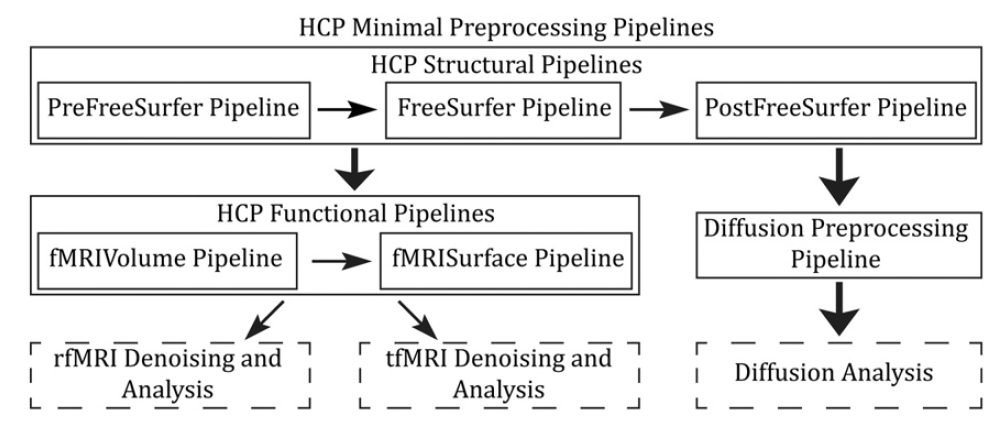
\includegraphics[width=\linewidth]{hcp_preprocessing_overview}
   \captionof{figure}{HCP Preprocessing Pipelines Overview}
   \label{fig:hcp_pipelines_overview}
   \caption*{Extracted from \cite{Gla13}}
\end{center}

Out of the six pipelines illustrated in Figure \ref{fig:hcp_pipelines_overview}, we used three structural pipelines and one functional pipeline for study. The pipelines are listed below, 
\begin{itemize}
  \item PreFreeSurfer
  \item FreesSurfer
  \item PostFreeSurfer
  \item fMRIVolume
\end{itemize}

The HCP pipeline is open sourced, and we used the version 3.19.0\footnote{\url{https://github.com/Washington-University/Pipelines/releases/tag/v3.19.0}} for our study. The details of pipeines are listed below. 

\subsubsection{PreFreeSurfer}
Main goals of, PreFreeSurfer, according to~\cite{Gla13} are, 1) to produce an undistorted ``native" structural volume space for each subject; 2) align the T1W and T2W images; 3) perform bias field correction; 4) register the subject's native structural volume space to MNI space. The workflow of PreFreeSurfer is illustrated in Figure \ref{fig:prefreesurfer_overview}.

\begin{center}
  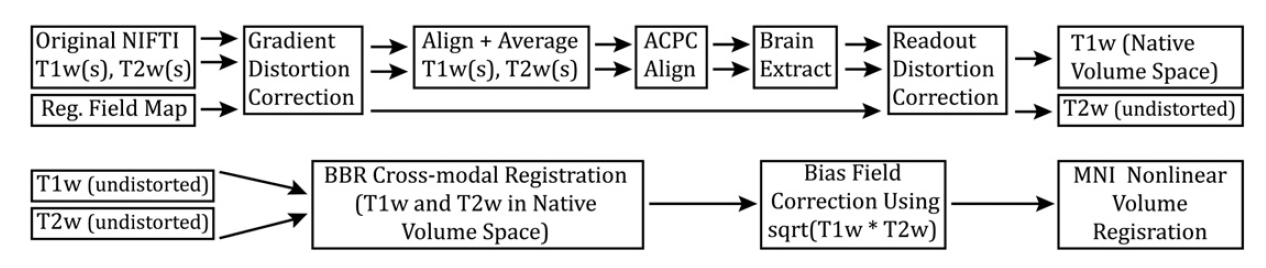
\includegraphics[width=\linewidth]{PreFreeSurfer_Architecture}
  \captionof{figure}{PreFreeSurfer Overview}
  \label{fig:prefreesurfer_overview}
  \caption*{Extracted from \cite{Gla13}}
\end{center}

PreFreeSurfer starts with correcting the distortions caused by magnetic resonance gradient nonlinearity~\cite{Gla13}. According to~\cite{Zou2004}, ``Gradient nonlinearity is a static characteristic of the gradient coil system known to system engineers and universally utilized for correction of geometric distortions for routine MRI scans". All images used in structural processing (T1w, T2w, the field map and phase) must be corrected from gradient nonlinearity distortion. The correction is done with a customized version of gradient\_nonlin\_unwarp package available in FreeSurfer. As per the definition given by~\cite{t1w_t2w}, T1-weighted images provides good contrast between gray matter and white matter in brain while cerebrospinal fluid is void of signal (black color) and T2-weighted images provides good contrast between cerebrospinal fluid and brain tissue. Figures~\ref{fig:T1w} and~\ref{fig:T2w} illustrates T1-weighted and T2-weighted images.\\

\begin{center}
  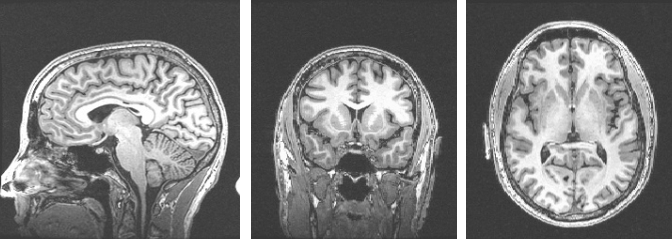
\includegraphics[width=\linewidth]{T1_v3}
  \caption{T1-weighted image}
  \label{fig:T1w}
  \caption*{Extracted from \cite{t1w_t2w}}
\end{center}

\begin{center}
  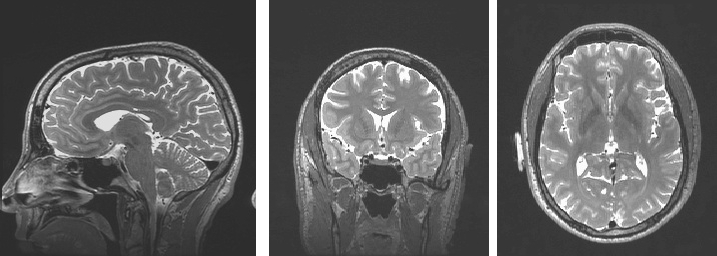
\includegraphics[width=\linewidth]{T2_v1}
  \caption{T2-weighted image}
  \label{fig:T2w}
  \caption*{Extracted from \cite{t1w_t2w}}
\end{center}

Next step is aligning the T1w and T2w images, using FSL's FLIRT. Subsequent step is aligning the average T1w and T2w images to the MNI space template. The main purpose behind this step is to have the same orientation as the template for the ease of visualization.

After this ACPC alignment step, a robust initial brain extraction step is performed using FSL's linear (FLIRT) and non-linear (FNIRT) registration. Removing the readout distortion is the last step in creating the subject's undistorted native volume space. Readout distortion is caused when the digital data is retrieved from an electronic medium and is is displayed in a human understandable format.

For correcting the gradient nonlinearity distortion, the images are converted into a field map using the fsl\_prepare\_fieldmap\_script. According to \cite{field_map}, ``A field map is an image of the intensity of the magnetic field across space". Mean magnitude and field map images are corrected for gradient nonlinearity distortion. The field map is then transformed according to these registrations and used to unwarp the T1w and T2w images, removing the differential readout distortion present in them. The readout-distortion-corrected T1w image, which now has all spatial distortions removed from it, represents the native volume space for each subject. The undistorted T2w image is cross-modally registered to the T1w image using FLIRT's boundary based registration (BBR) cost function. Boundary based registration focus on aligning intensity gradients across tissue boundaries. Once T1w and T2w images are in the same space , intensity inhomogeneity correction is applied on these images. After the bias field correction , T1w image is registered to MNI space after a FLIRT registration followed by FNIRT nonlinear registration.

The output of PreFreeSurfer pipeline are organized into a folder called T1w that contains native volume space images and a second folder (MNINonLinear) that contains MNI space images~\cite{Gla13}.

\subsubsection{FreeSurfer}
HCP pipelines uses FreeSurfer version 5.2 with a lot of enhancements made particulariy focusing HCP data. The main goals, according to~\cite{Gla13} are, 1) improve the robustness of brain extraction; 2) fine tune T2w to T1w registration; 3) accurately place the white and pial surface with high resolution data; 4) perform FreeSurfer's standard folding-based surface registration to their surface atlas (fsaverage). The workflow of FreeSurfer is illustrated in Figure~\ref{fig:freesurfer_overview}.

\begin{center}
  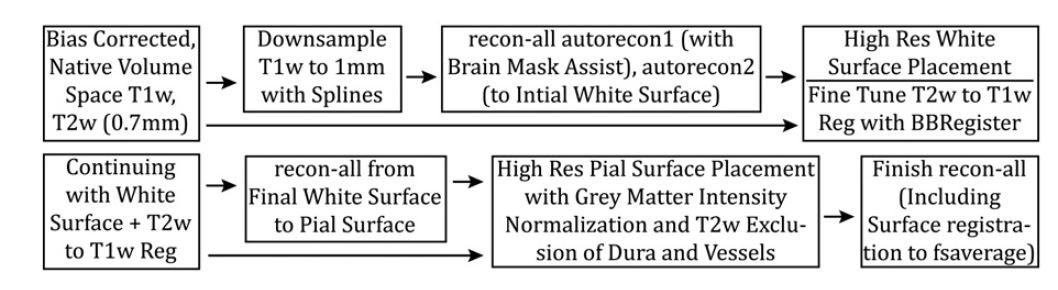
\includegraphics[width=\linewidth]{FreeSurfer_Architecture}
  \captionof{figure}{FreeSurfer Overview}
  \label{fig:freesurfer_overview}
  \caption*{Extracted from \cite{Gla13}}
\end{center}

After the PreFreeSurfer processing, FreeSurfer's recon-all pipeline is used for processing the output from the PreFreeSurfer pipeline. Recon-all pipeline is not able to process structural images having high resolution. So HCP data is downsampled to meet the requirements of the recon-all pipeline.

The T1w registration in the FreeSurfer is aided using the initial brain mask generated in PreFreeSurfer. The important steps that takes place before the recon-all process includes, automated segmentation of the T1w volume and tessellation and topology correction of the initial white matter surface. The resultant white matter surface is generated using a segmentation of the 1 mm downsampled T1w image.

The white matter surface placement is done using the original high resolution T1w images. The FreeSurfer volume and surface files brought into the .7 mm native volume space, the high resolution T1w volume is intensity normalized and the white matter surface position is adjusted based on intensity gradients in the .7 mm T1w image.

The T2w to T1w registration is fine-tuned using FreeSurfer's BBRegister algorithm. The corrected white matter surfaces are then brought back into FreeSurfer space and recon-all processing continues.

Next step is the generation of the Pial surfaces. The initial pial surfaces are generated from the high-resolution PreFreeSurfer bias-corrected T1w image.
The T2w images are used to remove any dura and blood vessels present in the image.

\subsubsection{PostFreeSurfer}
Main goals of, PostFreeSurfer, according to~\cite{Gla13} are, 1) produces all of the NIFTI volume and GIFTI surface files necessary for viewing the data in Connectome Workbench,2) application of surface registration; According to \cite{DBLP:journals/corr/HrgeticP13}, ''task of the surface registration algorithms is to determine the corresponding surface parts in the pair of observed clouds of 3D points, and on that basis to determine the spatial translation and rotation between the two views"; 3) downsampling registered surfaces for connectivity analyses; 4) creating the final brain mask, and creating myelin maps. Figure \ref{fig:postfreesurfer_overview} illustrates the workflow of PostFreeSurfer.\\

\begin{center}
  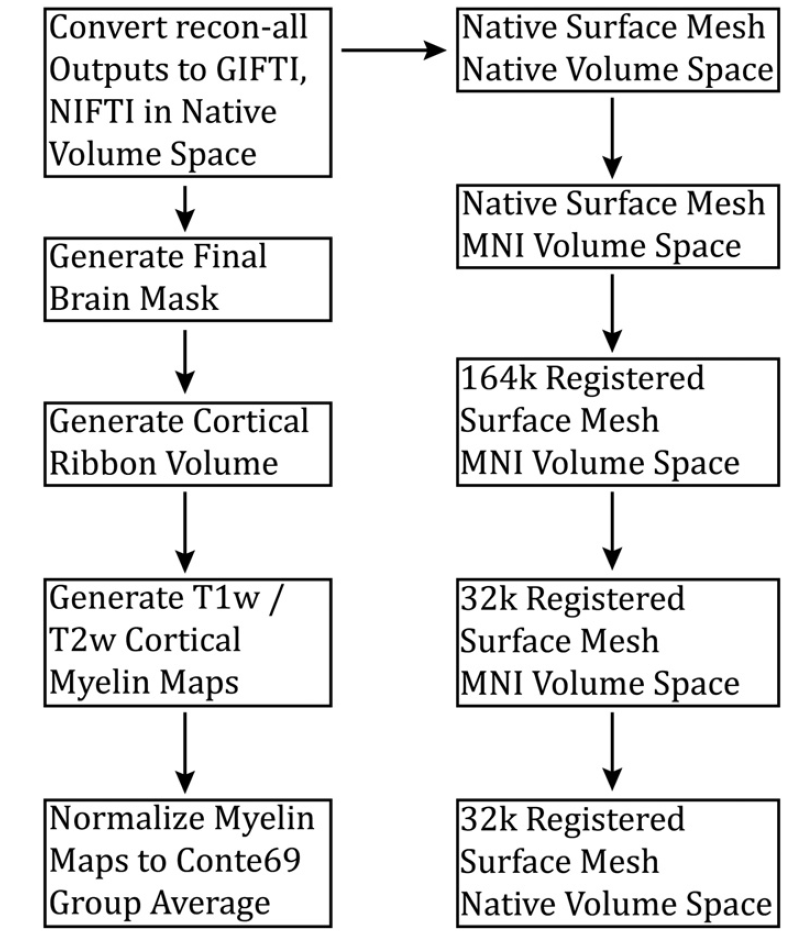
\includegraphics[width=\linewidth]{PostFreeSurfer_Overview}
  \captionof{figure}{PostFreeSurfer Overview}
  \label{fig:postfreesurfer_overview}
  \caption*{Extracted from \cite{Gla13}}
\end{center}

\subsubsection{fMRIVolume}
Main goals of, fMRIVolume, according to~\cite{Gla13} are, 1) remove spatial distortions; 2) realignment of volumes to adjust subject motion; 3) registration of fMRI data to structural volume; 4) normalizaton of the 4D image; 5) mask the data with final brain mask. Figure \ref{fig:fMRIVolume_overview} illustrates the workflow of fMRIVolume pipeline.\\

\begin{center}
  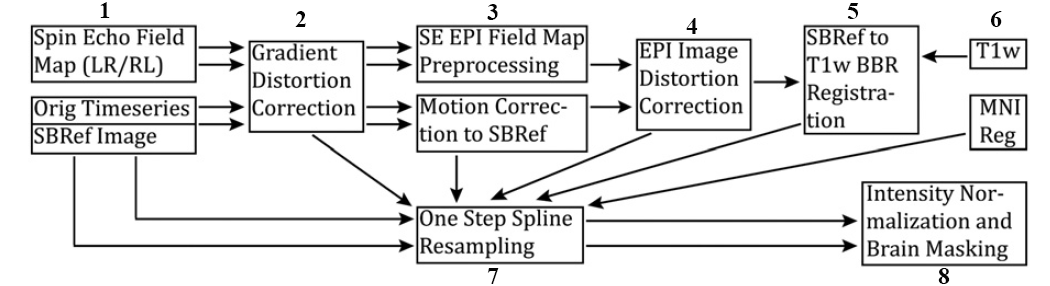
\includegraphics[width=\linewidth]{fMRI_Volume}
  \captionof{figure}{fMRI Volume Overview}
  \label{fig:fMRIVolume_overview}
  \caption*{Extracted from \cite{Gla13}}
\end{center}

\section{Pipeline Encapsulation}
A wrapper script\footnote{\url{https://github.com/big-data-lab-team/Dockerfiles-HCP-PreFreesurfer/blob/master/PreFreeSurfer-DockerFiles/command-line-script.sh}} was written on top of the HCP Pipelines to have the features which are listed below. 
\begin{itemize}
  \item Compute the checksum of the files in each subject before and after the execution
  \item Create execution directory and copies the subject to prevent corrupting the input data
  \item Record all the software (library versions) present in the container and hardware specifications of the workstation
  \item Ability to trace the execution using Reprozip (optional)
\end{itemize}

The checksums were computed before and after execution so that we can crosscheck them under different conditions to understand if there are any differences. These checksums are the primary criterion we use to find out if the files are having differeces. The execution directory creation copies the subject folder and thus it prevents the corruption of the HCP data. Another feature, recording of the software library versions and hardware specifications are done in order to make sure that the only factor that changes in these experiments is the operating system version. The optional Reprozip tracing feature is used to record the details of the HCP Processing.

\section{Pipeline Deployment}
The Docker container containing the HCP Pipeline along with the Boutiques descriptor was deployed on a server setup as part of our study. With the help of CBRAIN along with the containers and the descriptors, we were able to process HCP subjects. Single server was used in order to prevent differences occuring in the files due to differences arising from the hardware architecture. Boutiques descriptors used for deploying the HCP Pipelines on CBRAIN is available at \cite{HCP_descriptors}.

%\begin{itemize}
 % \item Single server to ensure no hardware differences
  %\item Able to process multiple subjects at once
  %\item CBRAIN HCP plugins available here
%\end{itemize}

\section{File comparisions across conditions}
Repro-tools framework compares the files across different conditions based on checksum of files. HCP subjects processed under different conditions are kept in different directories. The basic check is making sure that the files are common to all conditions for comparision. A pair of condition is taken at a time for comparison. The checksum of the files are recorded before and after the processing. Repro-tools can compute the checksums locally as well. 

Two types of differences can occur due to the minimal preprocessing. One is inter-OS difference which occur due the the operating system library updates and the other type, intra-OS differences occur due to pseudo-random processes used in the pipelines. Repro-tools can be used to identify both kind of differences.

The first step is identification of files with differences in their checksums. For the files that are identified to have differences, different kind of metrics are used base on the file type to quantify the differences. Normalized root mean square error, Dice Coefficient, Text filter etc. are the various metrics used for quantifying the differences. Section \ref{sec:num1} explains the metrics in detail. 

These metric values help us understand how big or small the differences are. Apart from quanitfying the differences using type specific metrics, Repro-tools can also be used to trace the provenance of these differences. It is able to identify all the processes and associated parameters. These detailed information is helpful in debugging since we can recreate the processing step by step and identify the processes that creates the differences.

%\begin{itemize}
 %\item Identify the files that are common to all subjects and all conditions
 %\item Check intra-OS variability (e.g., due to pseudo-random processes)
 %\item Identifies files with differences (based on md5 checksum)
 %\item Associates file types with specific metrics (Normalized RMSE, Text filters, Dice coefficient)
 %\item Computes difference matrix for each metric and associates matrix with Reprozip trace
%\end{itemize}

\section{Provenance Capture}
According to~\cite{Ikeda:2010:PSP:1855795.1855800}, ``provenance captures where data came from, how it was derived, manipulated, and combined, and how it has been updated over time". Provenance information can be used to explain the source or evolution of a data set. Thus it can help in generating a deeper understanding of the data set. It can also be used to verify and confirm that there were no bugs in the processing. Provenance information can be used to identify the bugs in the processing. Thus it can help in recomputing the steps that got corrupted and send the corrected data downstream~\cite{Ikeda:2010:PSP:1855795.1855800}.

The data recorded by Reprozip is recorded in an SQLite\footnote{\url{https://www.sqlite.org/}} database. Repro-tools framework queries this database to find out the provenance information about the files that has a difference in their checksum. Figure \ref{fig:provenance-query} contains the query used for finding the provenance information.\\

\begin{tcolorbox}[colback=black!5!white,colframe=black!75!black]
SELECT DISTINCT executed\_files.name, executed\_files.argv, executed\_files.envp, executed\_files.timestamp, executed\_files.workingdir from executed\_files INNER JOIN opened\_files where opened\_files.process = executed\_files.process and opened\_files.name like ? and opened\_files.mode=2 and opened\_files.is\_directory=0',('\%/'+file\_name,)
\end{tcolorbox}
\captionof{figure}{Query for provenance information}
\label{fig:provenance-query}

Query makes use of details about the 1) processes that wrote the file; 2) command line arguments used by those processes; 3) Environment variables used; 4) timstamp; 5) working directory. By the help of the details we get out of the query, we can reproduce the steps to debug the processes that create these differences.

\section{Metrics} \label{sec:num1}
The metrics that are used to quantify the differences are described below.

\subsection{Normalized Root Mean Sqaure Error (NRMSE)}
As defined in \cite{khosrow2017handbook}, ``The Root Mean Square Deviation (RMSD) or root-mean-square error (RMSE) is a frequently used measure of the difference between values predicted by a model or an estimator and the values actually observed". Normalizing the RMSD value makes it easier to compare between models or datasets.

Example from \cite{NRMSE}, the RMSE of predicted values ${\displaystyle {\hat {y}}_{t}}$  for times t of a regression's dependent variable ${\displaystyle y_{t}}$ is computed for n different predictions as the square root of the mean of the squares of the deviations:\\

\begin{center}
  \begin{equation}
     RMSE = {\sqrt {\frac{1} {n}{\sum\limits_{t = 1}^n {(\hat{y}_{t} - {y}_{t} } })^{2} } }
  \end{equation}
\end{center}

\begin{center}
  \begin{equation}
    NRMSE = {\frac{RMSE} {y_{max} - y_{min}}}
  \end{equation}
\end{center}

\subsection{Dice Similarity Coefficient}
Dice Similarity Coefficient can be used as a statistical validation metric for measuring the reproducibility of magnetic resonance images~\cite{Zou2004}. 
\begin{center}
  \begin{equation}
     J(A,B) = {{|A \cap B|}\over{|A \cup B|}} = {{|A \cap B|}\over{|A| + |B| - |A \cap B|}}
  \end{equation}
\end{center}
\begin{itemize}
\item NRMSE
\item Dice
\end{itemize}
